\chapter{Proof of concept, praktische Anwendung}\label{chap:experiments}
Die lokale Auswertung persönlicher Daten ist das Hauptargument für eine dezentralisierte Smart Home Steuerung aus Sicht des Konsumenten, die wie in der Befragung des IDC einsehbar ist \cite{IDC}, häufig angeben, dass die mögliche Auswertung ihrer Informationen durch dritte ein ausschlaggebender Faktor gegen die Anschaffung eines solchen Systems ist. Der Aufbau dieser Arbeit sieht entsprechend vor, zur Analyse der Daten die isolierten Logs eines einzelnen Smart Homes heranzuziehen und die Datenanalyse vollständig innerhalb des Heimnetzes des Anwenders durchzuführen, sich also auf eine „Small Data“ Analyse zu beschränken und so den Einwänden, die mit „Big Data Mining“ einhergehen, vorzugreifen. 

Um den theoretisch skizzierten Anwendungsfall praktisch zu untersuchen, wird der gewählte Process Mining Algorithmus auf einem einfachen, im lokalen Netz erreichbaren Server als Dienst implementiert. Dieser wartet auf den Eingang von Eventlogs aus einem Smart Home, verarbeitet die Rohdaten und leitet das resultierende Modell an eine Mobile Anwendung weiter. Die Anwendung soll dann dem Anwender die Möglichkeit geben, die vom Process Mining Algorithmus extrahierte Regel im Smart Home zu integrieren. Wird die Regel vom Nutzer akzeptiert, übernimmt der lokale Server die Implementation der Aufgaben auf den relevanten vernetzten Geräten.

\section{Aufbau und Komponenten der praktischen Anwendung}
Das Smart Home Modell, welches zu Testzwecken dieses Projektaufbaus dient ist Teil des Inventars des ITOM Instituts und mit einer Auswahl an Sensoren und Aktoren ausgestattet. 
Desweiteren wird die im Rahmen einer, zuvor am ITOM Institut entstandenen, Bachelorarbeit Android Anwendung „Grafischer Regeleditor“ als Basis für die Kommunikation mit dem Anwender genutzt und um die Funktion der automatisierten Regelerkennung erweitert. Die Funktionalität der Kommunikation mit einem lokalen Server und das manuelle Anlegen von Regeln für iot Geräte ist bereits in der genannten App integriert.

Das Process Mining, die Archivierung der Eventlogs und die Kommunikation mit den vernetzten Geräten des Smart Homes wird von einem einfachen Server übernommen, in diesem Fall wird ein Raspberry Pi 3.0 eingesetzt. Um den Anwender über neue erkannte Muster zu informieren, wird jeweils eine Benachrichtigung an das Mobiltelefon versandt, das Versenden der Benachrichtigung wird vom ‚firebase‘\footnote{https://firebase.google.com/} Dienst übernommen, diese Aufgabe kann um den Aspekt der Datensicherheit fortzusetzen ebenfalls von einem lokalen Dienst erfüllt werden.

\section{Dienste und Skripte auf dem Heimserver}
Da die Anwendung auf der Architektur des Projekts ‚Graphischer Regeleditor‘ aufbaut, wird in dieser Arbeit vorausgesetzt, dass openHab als Dienst im Heimnetzwerk des Anwenders verfügbar ist, da dieser für die Aufgabe der Kommunikation mit den iot Geräten, welche die Einträge für das Process Mining notwendige Ereignislog erstellen, verantwortlich ist. 

Die quelloffene openHAB (open Home Automation Bus) Automatisierungssoftware implementiert eine weite Bandbreite herstellerabhängiger Standards und gewährleistet somit eine Kommunikation zwischen den Technologien bzw. Sensoren. Die openHAB-Software stellt 12 Dienste zur Verfügung, um die von den Sensoren gemessenen Daten zu persistieren. Die Automatisierungslogik der openHAB-Software ist als einfacher Regex-Agent anzusehen. 
Um die Brücke von der unverarbeiteten gesammelten Menge an Ereigniseinträgen zu einer neuen, automatisiert erkannten Regel zu schlagen wird ein Script auf dem Server hinterlegt, welches periodisch alle notwendigen Teilschritte des Prozesses aufruft. Jeweils am ersten Tag jedes Kalendermonats wird die auf dem lokalen Server angelegte Ereignislog geladen und zunächst vom .csv (Comma seperated values) in das .xes Format konvertiert. 

Diese Konvertierung ist ein simpler Vorgang, bei dem jeder Eintrag, der in der csv Datei eine einzelne Instanz einer Aktion eines IoT Geräts repräsentiert, in seine Komponenten gespalten und ins XES Format übertragen wird. Die Komponenten umfassen, wie eingangs beschrieben, den Zeitstempel, den Namen des Geräts - in der Form in der er unter openHab hinterlegt ist - sowie die Aktion oder den Sensorwert der den Eintrag erzeugt hat. Diese Komponenten werden im Ausgangsformat von sog. XML-Tags eingeschlossen, die eine Beschreibung des Inhalts enthalten, so wie es der XES Standard vorsieht. Dieser Schritt erleichtert Mining Algorithmen den Umgang mit der Eingangsdatei. 

%Bei der Untersuchung von unverarbeiteten Eventlogs, die im Smart Living Modellhaus des ITOM Institus entstanden sind, ist erkennbar, dass es bei einigen der im Haus integrierten Geräte dazu kommt, dass sie ein Zeitstempelformat nutzen, welches die Sekunden nicht angibt. Hier ist also vor der Konvertierung ein Vorverarbeitungssschritt notwendig, der über jede Zeile iteriert und die Stempel einander angleicht. Da kein universeller Standard für IoT Logs Branchenweit akzeptiert wird und die Hersteller diese beliebig formatieren können, sind mit jedem weiteren angeschlossenen Gerät auch weitere Abweichungen von der erwarteten Form nicht auszuschließen. Um diesem Problem entgegenzuwirken können Tools wie ‚syslog-ng‘ eingesetzt werden, die in der Lage sind die meisten Formen von Eventlogs auf ein einheitliches Format zu bringen.

Im nächsten Schritt ruft das Script ein in der Programmiersprache Java geschriebenes Programm auf, welches Process Mining auf dem neu entstandenen XES Dokument durchführt. Konkret wird dafür ProM auf dem Server gestartet und das Inductive Visual Miner Plugin ausgewählt.
Das Inductive Visual Miner Plugin erlaubt es Prozessmodelle in Eventlogs mithilfe des Inductive Miners zu entdecken. Über die GUI des Plugins können auch Vorverarbeitungsschritte vorgenommen werden, um Rauschdaten zu unterdrücken oder weitere Attribute zur Berücksichtigung bei der Datenanalyse auszuwählen, falls diese im Log gegeben sind. Der Vorverarbeitungsschritt der Rauschreduzierung ist unerlässlich für die Regelfindung. Es sollten keine Knoten als Teil des Regelvorschlags an den Nutzer gelangen, die nicht definitiv auch Teil seines regulären Ablaufs sind. 

\begin{figure}[!h]
    \centering
    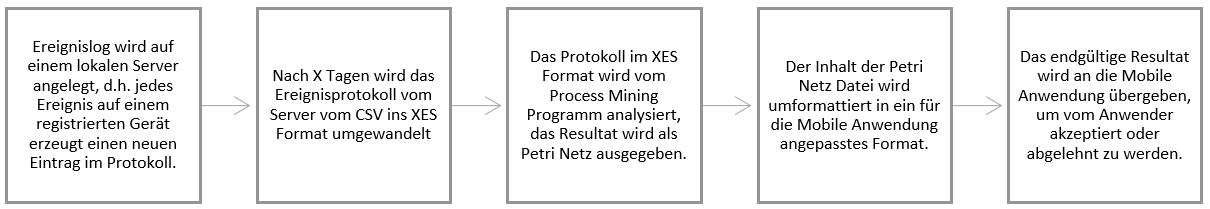
\includegraphics[width=1.2\textwidth,origin=c]{figures/Appbildungen/pipeline.PNG}
    \caption{Verarbeitungsschritte zur Auswertung der Smart Home Daten}
    \label{fig:4}
\end{figure}

In dieser Arbeit wird der Schwellwert für Rauschdaten über einen iterativen Prozess gesucht. Da es im Vorfeld keine Information über die Menge der Rauschdaten im zu untersuchenden Eventlog geben kann, wird wie folgt verfahren. 

Ziel ist es ein Modell der häufigsten und kurzen Routinen zu finden. Genauer soll eine Regel mindestens eine Vorbedingung und eine Aktion enthalten, maximal drei Vorbedingungen werden akzeptiert. Nachdem ein Modell aus zwei Knoten gefunden wurde wird nur dann um einen weiteren Knoten erweitert, wenn dieser genauso häufig Teil des Ablaufs ist wie die bisherigen Elemente. Der Regler für den Rauschmengenschwellwert (im Plugin 'activities' genannt) wird mit einem Startwert von 0.001 belegt, ein Petri Netz erzeugt und dessen Knoten gezählt. Es wird solange um 0.001 addiert, bis zwei Knoten ein Modell binden und ihre Häufigkeit im Gesamtlog in einer Variable gespeichert. Der Schwellwert wird weiter um 0.001 addiert, bis ein weiteres Element in das Modell aufgenommen wird. Hat sich die Häufigkeit dieses Modells im Vergleich zum Vorangegangen reduziert, wird das Modell aus zwei Knoten als korrekte Regel akzeptiert, wenn nicht wird weiter Verfahren bis ein weiterer Knoten erscheint und die Häufigkeiten und wie im vorangegangen Schritt verfahren.
Ist dieser Schritt abgeschlossen, ist eine Regel gefunden worden.
Das Modell des Miners wird in ein PNML Format übertragen, welches Petri Netze nach dem XML Schema beschreibt.

Abschließend enthält das Script einen Aufruf eines kurzen in Python geschriebenen Programms, welches den Firebase Dienst dazu auffordert eine Benachrichtigung an das Mobile Gerät des Anwenders zu senden, welche den Inhalt des PNML Dokuments enthält.

\section{Mobile Anwendung als Steuerungs- und Kommunikationsschnittstelle}

Um die Regeleditor Anwendung um die Kommunikation mit einem dedizierten Firebase Dienst zu erweitern, wird eine Klasse PMFireBaseMessagingService angelegt, welche im Anhang hinterlegt ist. \todo{ Ref und Die Authentifizierung erfolgt über ein token system ...}

Gleichzeitig ist diese Klasse verantwortlich dafür die Regel entgegenzunehmen und übergibt Sie in die an die im Rahmen dieser Arbeit erzeugte PMRule Klasse, welche verantwortlich für das Parsen des empfangenen Textes in eine Regelform ist. Konkret wird dies von der Funktion parseReceivedRule() übernommen.

\begin{lstlisting}[language=Java]
       private void parseReceivedRule(JSONArray ruleJSON) throws JSONException {
        PMRule r = new PMRule();
        int lastEntry = 0 ;
        for(int j=0;j<ruleJSON.length();j++){
            Log.d("processmining", "rules Array"+j+": "+ruleJSON.getJSONArray(j));

            if(ruleJSON.getJSONArray(j).length()>1){
                lastEntry = ruleJSON.getJSONArray(j).length()-1;
                Vector<String> preconditions = new Vector<>();
                for(int i=lastEntry; i>=0;i--){
                    if(i==lastEntry)
                        r.setAction(ruleJSON.getJSONArray(j).getString(i));
                    else
                        preconditions.add(ruleJSON.getJSONArray(j).getString(i));
                }
                r.setPrecondition(preconditions);
                PMRules.add(r);
                Log.d("processmining", "IF: "+r.getPrecondition()+" THEN: "+r.getAction());
            }
        }
        Intent pmIntent = new Intent(Main.this, ProcessMiningRuleActivity.class);
        pmIntent.putExtra("IF", r.getPrecondition());
        pmIntent.putExtra("THEN", r.getAction());
        startActivity(pmIntent);
    }
\end{lstlisting}

\begin{wrapfigure}{R}{0.5\textwidth}
  \begin{center}
    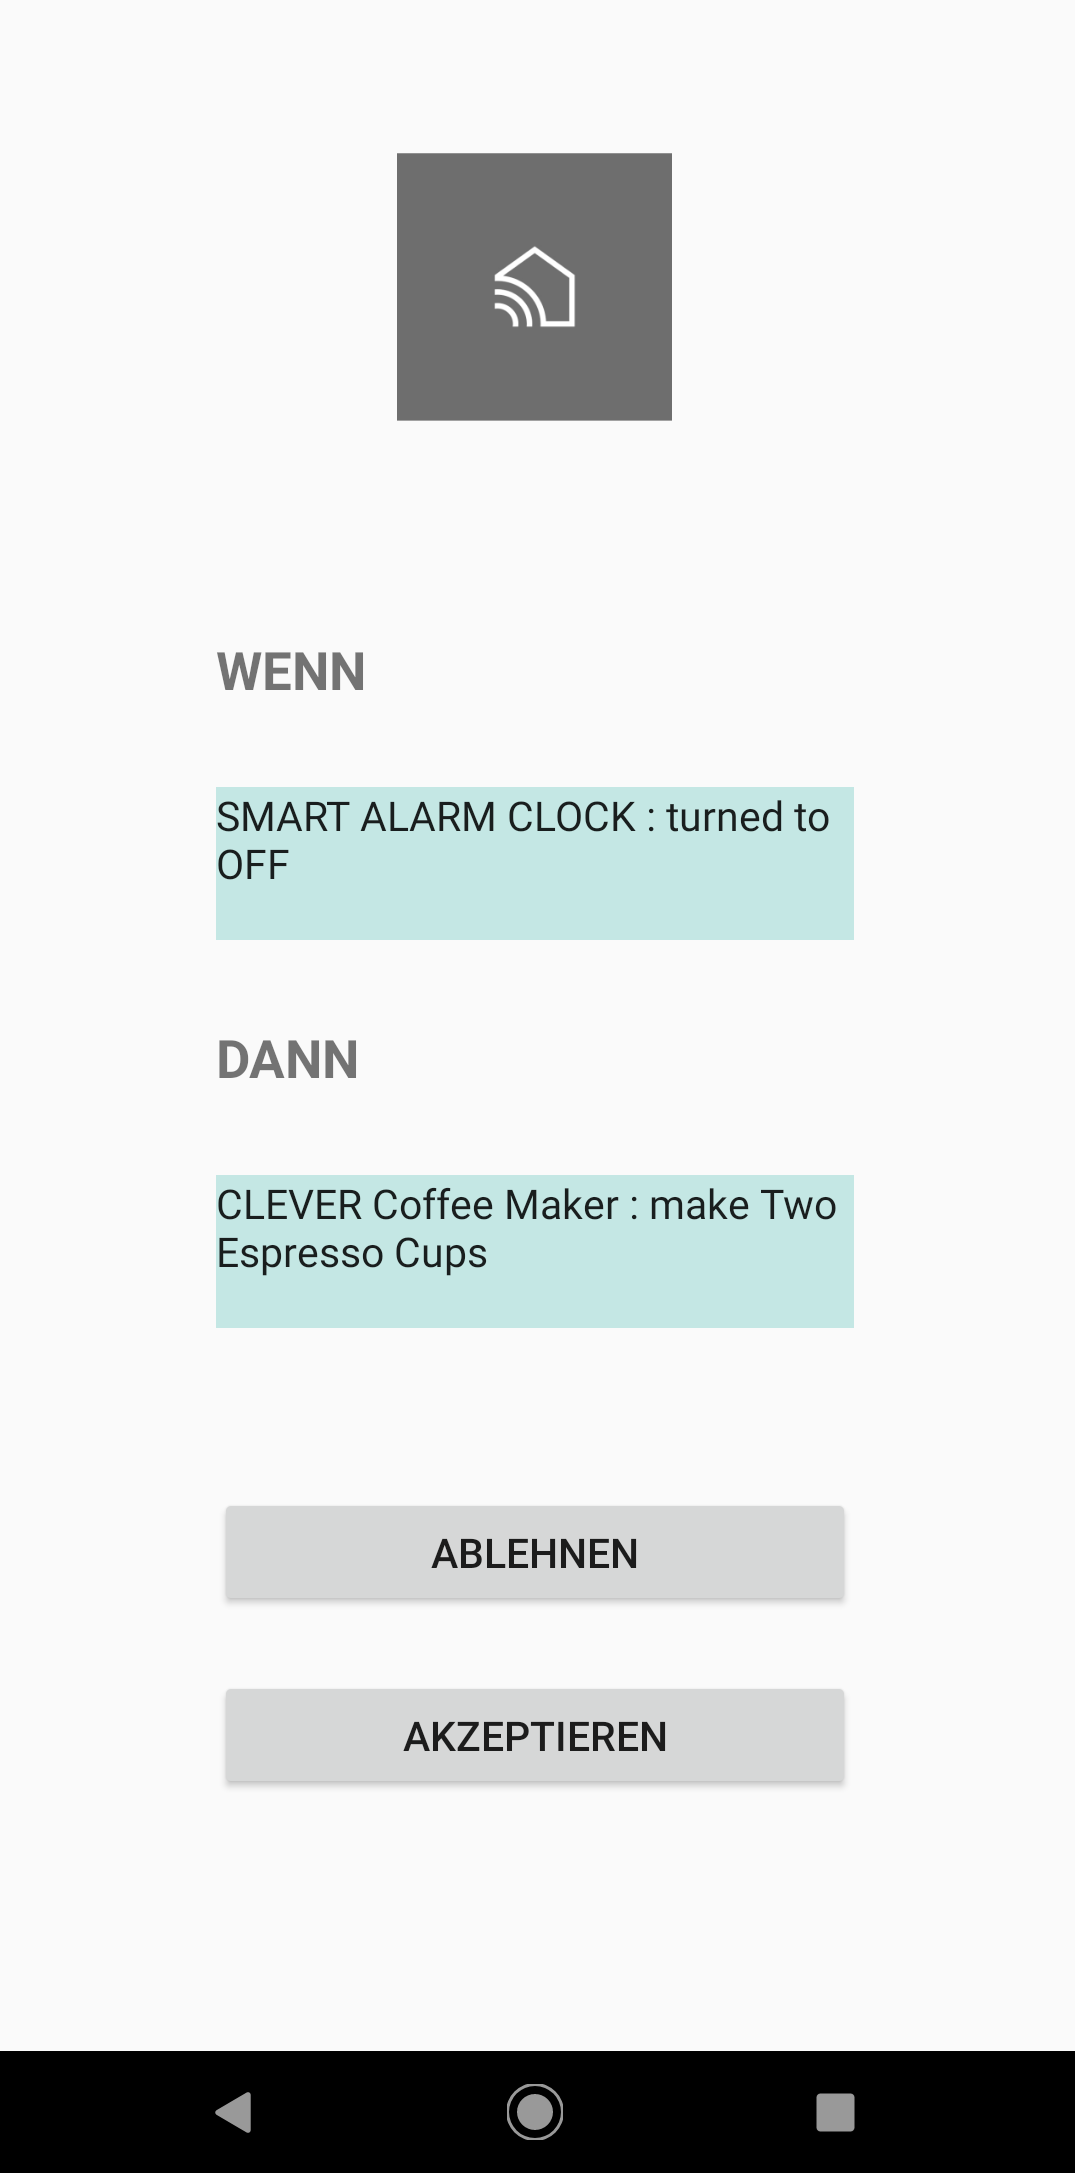
\includegraphics[width=0.3\textwidth]{figures/Appbildungen/newRuleDialog.png}
  \end{center}
  \label{fig:appdialog}
  \caption{Proof of Concept: Dialog bei Eingang neuer erkannter Regel}
\end{wrapfigure}

Nachdem der Endanwender die Benachrichtigung auf dem Mobilen Gerät anwählt, wird ein Dialog innerhalb der „Grafischer Regeleditor“ Anwendung gestartet. Ein Beispiel ist auf Abbildung \ref{fig:appdialog} zu sehen. Die Vorbedingungen und Aktionen der Regel werden im Wenn – Dann Format dargestellt. Der Nutzer hat zunächst die Möglichkeit die Regel zu akzeptieren oder abzulehnen. Wird sie abgelehnt, wird die Regel nicht ins lokale openHab System aufgenommen und eine Feedback Nachricht an den Server übermittelt. Dies soll verhindern dass eine ungewünschte Regel wiederholt vorgeschlagen wird. Der Server soll neue Regeln zunächst gegen bestehende und abgelehnte abgleichen, bevor eine neue Anfrage gestellt wird.

Wird der Vorschlag vom Anwender akzeptiert, wird er zu einem weiteren Fenster weitergeleitet, welches ihm die Option bietet, die Regel ohne Anpassungen zu übernehmen, oder aber die vorgeschlagene Regel zu editieren. Beispielsweise können weitere Vorbedingungen oder Aktionen hinzugefügt oder entfernt werden, für diese Funktionalität wird auf das Regelwerk der zur Verfügung gestellten „Grafischer Regeleditor“ App zurückgegriffen. 
Nachdem die Regel vom Nutzer akzeptiert worden ist, wird sie wie in der Vorgängerversion der Anwendung auch in die sqLite Datenbank eingetragen. openHab empfängt die aktualisierte Datenbank und wird nun die Aktion ausführen, sobald die vermerkten Vorbedingungen erfüllt sind.
Weitere Funktionen wie das nachträgliche Entfernen oder Editieren der Regeln stehen dem Anwender wie bereits in der Vorgängerversion zur Verfügung.
Dieser Prozess ist in Abbildung \ref{fig:Kommunikationsablauf} noch einmal im BPMN Format graphisch dargestellt.



\begin{figure}[!ht]
    \centering
    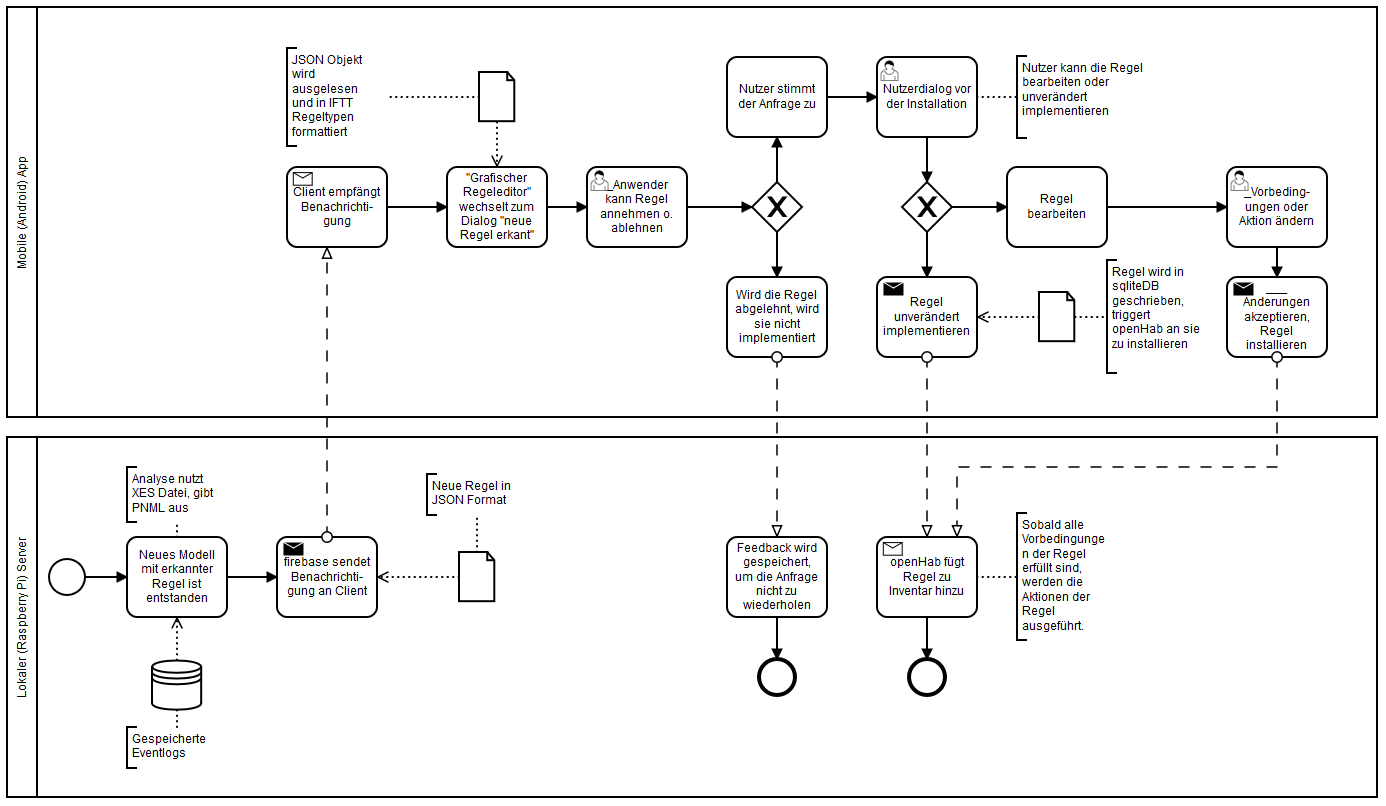
\includegraphics[width= 1.52\textwidth, angle=90,origin=c]{figures/Appbildungen/diagramm_app.PNG}
    \caption{Ablauf der Kommunikation zwischen Endanwender und lokalem Server}
    \label{fig:Kommunikationsablauf}
\end{figure}